

\subsection{Metrics}

In the next sections we will introduce the Framework for Distributional Reinforcement Learning. Before, we were only dealing with real numbers, now we will work on a space of Distribution. To do it properly, we need to introduce a few metrics.
\subsubsection*{Wasserstein Metric}

\begin{definition}[Wasserstein Metric\cite{rowland_analysis_2018}]
    Let $p \geq 1$ and $\PPPP_p(\RR)$ the space of distributions with finite $p^{\text{th}}$ moment. Let $\nu_1, \nu_2 \in \PPPP_p(\RR)$ and $\Lambda(\nu_1, \nu_2)$ the set of distribution on $\RR^2$ with marginals $\nu_1$ et $\nu_2$. The p-Wasserstein distance $d_p$ is then defined as :

    \[ d_p(\nu_1, \nu_2) = \left( \inf_{\lambda \in \Lambda(\nu_1, \nu_2)} \int_{\RR^2} |x-y|^p \ \dd\lambda(x,y) \right)^{\frac{1}{p}}\]

    Let $\eta_1, \eta_2 \in \PPPP_p(\RR)^{\XX \times \AAA}$. We also define the supremum-p-Wasserstein distance $\overline{d}_p$ by:

    \[ \overline{d}_p(\eta_1,\eta_2) = \sup_{(x,a) \in \XX \times \AAA} d_p(\eta_1^{(x,a)}, \eta_2^{(x,a)})\]
\end{definition}

This is the general definition, but it will not be practical to compute with. Instead, in our case, we have a simpler expression:

%définir la norme associé à une variable aléatoire (Bellemare)
\begin{lemma}[\cite{bellemare_distributional_2017}]
    Let $\nu_1, \nu_2 \in \PPPP_p(\RR)$ with respective cumulative distribution $F$ and $G$. Let $\UU$ be a uniform random variable on $[0,1]$. then 

    \[ d_p(\nu_1, \nu_2) = \norm{F^{-1}(\UU) - G^{-1}(\UU)}_p \]
    %\[ d_p(\nu_1, \nu_2) = \EE{\left(F^{-1}(\UU) - G^{-1}(\UU)\right)^p}^{\frac{1}{p}} \]

    which, in the case $p < \infty$ simplifies to:

    \[ d_p(\nu_1, \nu_2) = \left(\int_0^1\left|F^{-1}(u) - G^{-1}(u)\right|^p du\right)^{\frac{1}{p}} \]

\end{lemma}

$d_1$ is the one that will be used the most.

\paragraph{Cramer Distance}

\begin{definition}[\cite{rowland_analysis_2018}]
    Let $\nu_1, \nu_2 \in \PPPP(\RR)$. We define the family of metrics $\ell_p$ by :

    \[ \ell_p(\nu_1, \nu_2) = \left( \int_\RR (F_{\nu_1}(x) - F_{\nu_2}(x))^p \dd x\right)^{\frac{1}{p}} \]

    $\ell_2$ is called the Cramer distance.

    We also define the suppremum version of the $\ell_p$ norm:
    \[ \overline{\ell}_p(\eta_1,\eta_2) = \sup_{(x,a) \in \XX \times \AAA} \ell_p(\eta_1^{(x,a)}, \eta_2^{(x,a)})\]
\end{definition}

\begin{remark}
    $l_1 = d_1$
\end{remark}





\subsection{Distributional Reinforcement Learning}
%parler des résultats obtenus, pour motiver l’introduction de la notion, en plus de donner plus de possibilité sur le choix de l’optimisation.

In 2017, \cite{bellemare_distributional_2017}[Bellemare et al.] introduces the Distributional Reinforcemennt Learning framework. The idea is to compute the full distribution of the return instead of just the expected return. In his paper, they introduce the distributional Bellman operators and prove theoretical results on their properties.
\\%souligner en bleu à cause de retour à la ligne juste après une grosse expression qui prend plusieurs lignes.

The random return is the sum of the discounted random reward:

\begin{equation}
    Z(x,a) = \sum_{t = 0}^{\infty} \gamma R_t \ |\ X_0 = x, A_0 = a
\end{equation}

The idea is that the distribution of the reward would follow similar Bellman equations:

\begin{equation}\label{randvarbellman}
    Z(x,a) \deq R(x,a) + \gamma Z(X^\prime, A^\prime)
\end{equation}

with $X^\prime, A^\prime$ the random next state-action. 

\subsubsection*{Policy Evaluation}
Let’s consider a policy $\pi$. The distribution of the random return under $\pi$ will be written as follows:

\[ \eta_\pi^{(x,a)} = \text{Law}_\pi \left( \sum_{t = 0}^{\infty} \gamma R_t \ | \ X_0 = x, A_0 = a \right) \]

and we will write $\eta_\pi$ as the collection of distribution $(\eta_\pi^{(x,a)})_{(x,a) \in \XX \times \AAA}$.\\

What makes the distributional framework worth studying, is the generalization of the Bellman equation and its properties:
The random return associated to policy $\pi$ verifies the \emph{distributional Bellman equation}:
\[\eta_\pi = \TT^\pi \eta_\pi \]
where $\TT^\pi$ is the Bellman operator defined by:

\[
    \TT^\pi \eta^{(x,a)} = \int_\RR \sum_{(x^\prime,a^\prime)\in \XX \times \AAA} (f_{r,\gamma})_\#\eta^{(x^\prime,a^\prime)}\pi(a^\prime|x^\prime)p(r,x^\prime|x,a)dr
\]

with $(f_{r,\gamma})_\#\eta$ is the pushforward measure define by $f_\#\eta(A) = \eta(f^{-1}(A))$ for all Borel sets $A\subseteq R$ and $f_{r,\gamma}(x) = r + \gamma x$ for all $x \in R$.

While this operator seems more cumbersome that the non-distributional one, it just comes down to rewriting equation \ref{randvarbellman} for distributions. The proof use the exact same idea as in the non-distributional case, but in this new formalism. \\

In the tabular case, it is possible to solve this fixed point equation by matrix inversion. However, it doesn’t seem possible to do so when dealing with distribution. To solve it, we will use the following result, that is same used to solve the non-tabular non-distributional case.

Similarly as in the non-distributional case, this operator is a $\gamma$-contraction under a well chosen metric: the maximal $p$-Wasserstein metric $\overline{d}_p$ (for $p \geq 1$).

This result is very important in the sense where it gives an theoretical algorithm to compute the value distribution of a policy.

\[ \forall \eta \in \PPPP(\RR)^{\XX \times \AAA}, \quad (\TT^\pi )^n \eta \underset{n \rightarrow \infty}{\longrightarrow} \eta_\pi \]

The Wasserstein metric is important here because the same operator is not always a contraction under the total variation distance, the Kolmogorov distance or the Kullback-Liebler divergence. (ref in article de Bellemare)

Even though this algorithm seems promising, there are several issues that arise in practice, that make it difficult to implement: It is impossible to represent exactly all the space of distributions, which requires a parametrisation of the distribution and a projection step, then we most of the time don’t have access to the exact transition of the MDP, which requires a stochastic estimation of the Bellman Operator. Those issues will be tackled in the next subsections.

\subsubsection*{Control} 
Here, the goal still is to find an optimal policy. However, we will consider the full distributions of return to reach it.

We define by optimal distribution a distribution associated to an optimal policy: $\sta\eta \in \{ \eta_{\sta\pi} \ | \ \sta\pi \in \argmax_{\pi} \EEE{R \sim \eta_\pi}{R}\}$.
One of the first difference that we notice is the fact that there can be several different optimal distribution. Those optimal distribution all have the same mean, but a distribution having the optimal mean may not be an optimal distribution, because some distributions may not come from any (stationary) policy. [mettre les exemples]
 

As expected, the optimal distributions verify the optimal distributional Bellman equation: $\sta\eta = \TT\sta\eta$ with 

\[
    \TT\eta^{(x,a)} = \int_\RR \sum_{(x^\prime,a^\prime)\in \XX \times \AAA} (f_{r,\gamma})_\#\eta^{(x^\prime,\sta a(x^\prime))}p(r,x^\prime|x,a)dr
\]
where $\sta a(x^\prime) = \argmax_{a^\prime \in \AAA} \EEE{R \sim \eta^{(x^\prime, a^\prime)}}{R}$

The first interesting Control result is the fact that this operator is a contraction in average:

\begin{lemma}
    Let $\eta_1, \eta_2 \in \PPPP(\RR)^{\XX\times\AAA}$, we write $\EE{\eta}:= \EEE{Z \sim \eta}{Z}$. Then:
    \[ \norm{\EE{\TT\eta_1} - \EE{\TT\eta_2}}_\infty \leq \gamma \norm{\EE{\eta_1} - \EE{\eta_2}}_\infty \]  

    Which means that $\EE{\TT^n \eta} \underset{n \rightarrow \infty}{\longrightarrow} \sta Q$ exponentially quickly.
\end{lemma}

As before this leads to a theoretical algorithm to find the optimal value function using the whole distribution. We have another result regarding the convergence of the distribution itself:

\begin{theorem}
    Let $\XX$ and $\AAA$ be finite. Let $\eta \in \PPPP(\RR)^{\XX\times\AAA}$. Assume that there is a single policy $\sta \pi$. Then: 
    
    \[\TT^n \eta \underset{n \rightarrow \infty}{\longrightarrow} \eta_{\sta \pi} \text{ uniformly in } \overline{d}_p, \ p\geq1\]
\end{theorem}

This theorem is very important to understand how distributions behave. At first it seems really convenient, with the convergence of the distribution, but there are especially two points which are worth emphasizing. The first one is that there is no exponential convergence anymore and, in fact, the speed of the convergence is unknown. The second is the condition of unicity of optimal policy. While this condition seems reasonable, it is still possible to do without, at the cost of stationarity: if there are several optimal policy, the distribution converges uniformly to one associated to a possibly nonstationary optimal policy.

The non stationarity of the optimal policy isn’t an issue when the goal is solely to maximize the mean reward, as the greedy policy associated to its distribution will still be optimal. However, it can be more problematic if we try to find policy that takes acount of the whole distribution, such a safer or riskier policy.\\

The two previous properties are weaker that what we found in the Policy Evaluation case. To emphasize more on the differences, here are some more results that underline the pathologic cases that arise in Distributional Control:

\begin{proposition}
    The optimality operators are not always contractions.
\end{proposition}

\begin{proposition}
    The optimality operators do not always have fixed points.
\end{proposition}

The lack of contraction is the precise result that prevents us to get the same properties as in the non-distributional case or as in the distributional, especially the existence and unicity of a fixed point, and the exponential convergence.




















\subsection{Distribution Parametrization}

One of the main issue when dealing with distribution in practice, is the question of representation. It is not possible for a computer to represent the full extent of the distribution space. It is then necessary to restrain ourself on a parametrized space.

In their papers, \cite[Morimura et al.]{morimura_parametric_2012} decide to parametrize the return distribution as a Gaussian, a Laplace or a skewed Laplace distribution. Later, \cite[Bellemare et al.]{bellemare_distributional_2017} and then \cite[Dabney et al.]{dabney_distributional_2017} developed the theory for a richer class of parametric distributions, discrete ones, that are much more convenient. There two main approaches for that: the categorical approach, and the quantile regression approach.

\subsubsection*{Categorical}

This is the approach introduced by \cite[Bellemare et al.]{bellemare_distributional_2017} which led to the C51 algorithm that reached state of the art result for ALE. However, the theoretical properties of such approach were mainly developed later, by \cite[Rowland et al.]{rowland_analysis_2018}.

The idea is to use the hypothesis of bounded reward to use evenly spread diracs on that reward support, and use the diracs weight as the parameters.

\begin{figure}[!ht]
    \centering
    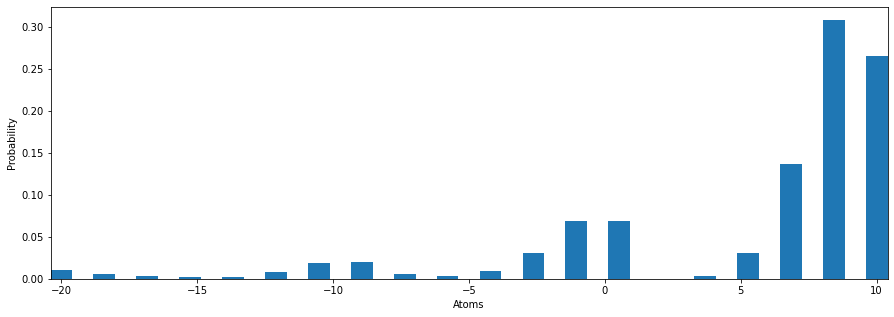
\includegraphics[height=0.2\textheight]{figures/personal_work/categoriacl.png}
    \caption{Example of a distribution projected by with the categorical approach}
\end{figure}

More formally, let’s consider $V_{\textsc{min}}, V_{\textsc{max}}$ the bounds for the reward, $N$ the number of diracs (the resolution) to use, $\Delta z = \frac{V_{\textsc{max}} - V_{\textsc{min}}}{N - 1}$ the steps between diracs. The support of the distributions will be $\{ z_i = V_{\textsc{\textsc{min}}} + i\Delta z \ |\ 0 \leq i < N \}$. The parametric family then is $\{ \sum_{i=0}^{N-1} q_i\delta_{z_i}  \ |\ \sum_{i=0}^{N-1} q_i = 1,\ 0\leq q_i \leq 1\}$.\\

%    We define the stochastic distributional Bellman operator $\hat\TT$ by :
%    \begin{align*}
%        (\hat\TT^\pi \eta_t)^{(x_t,a_t)} &= (f_{r_t,\gamma})_\#\eta_t^{%(x_{t+1}, \sta a)}\\
%        (\hat\TT^\pi \eta_t)^{(x,a)} &= \eta_t^{(x,a)} \qquad \text{if} (x,a) \neq (x_t, a_t)
%    \end{align*}
%    with $\sta a$ sampled from $\pi(\cdot|x_{t+1})$.

We define the projection operator $\Pi_C : \PPPP(\RR) \rightarrow \PPP_C$ by :

\begin{equation}
    \Pi_C(\delta_y) = 
    \begin{cases}
        \delta_{z_0} & y \leq z_0\\
        \frac{z_{i+1}-y}{z_{i+1}-z_{i}}\delta_{z_i} + \frac{y - z_i}{z_{i+1}-z_{i}}\delta_{i+1} & z_i < y < z_{i+1}\\
        \delta_{z_{N-1}} & y \geq z_{N-1}
    \end{cases}
\end{equation}
The idea behind is, for each atoms, to distribute their weight on the two closest of the projection, proportionnaly to how close they are.

Bellemare et al. introduced this projection step as an heuristic, without any theoretical motives or results related to the Wasserstein metric. It is Rowland et al. that later, found deep connection between this projection and another metric: the Cramer distance.

In fact, for the Wasserstein metric, we have the following result.
\begin{proposition}
    $\Pi_C\TT^\pi$ is not a contraction for $\overline{d}_p$ with $p > 1$.
\end{proposition}
For the case $p=1$ it is however true, but only because it is the same as the $\ell_p$ distance, for which we have much more properties:

\begin{proposition}
    For a specific subset of $\PPPP(R)$ and appropriate Hilbert space structure with $\ell_2$, $\Pi_C$ is the orthogonal projection of that subset onto $\PPP_C$
\end{proposition}
Even though the result is quite Abstract, it gives a beginning of explication on why the definition of the projection makes sense, and why it gives decent results. It also highlight the fact that this projection is closely related to the cramer distance. That distance indeed leads to better result and gives a contracting operator:

\begin{proposition}
    $\Pi_C\TT^\pi$ is a $\sqrt[p]\gamma$-contraction in $\overline{\ell}_p$.
\end{proposition}

The Banach fixed point theorem thus provides with a proof a convergence of the iterated projected Bellman operators:

\begin{equation}\label{ProjBellmanCatConv}
    \exists ! \eta_C \in \PPP_C^{\XX \times \AAA}, \ \forall \eta_0 \in \PPPP(\RR)^{\XX \times \AAA},\quad (\Pi_C\TT^\pi)^m\eta_0 \underset{m \rightarrow \infty}{\longrightarrow} \eta_C \quad \text{exponentially quickly in } \overline{\ell}_p
\end{equation}


It is important to notice that this does not have to converge to $\eta_\pi$, for the simple reason that this operator is convergent in the parametrized space $\PPP_C$, which may not contain $\eta_\pi$. The question that arises next, is how well does $\eta_C$ approximates $\eta_\pi$, question which was answered by \cite[Rowland et al.]{rowland_analysis_2018}.

\begin{lemma}
    Let $\eta_C$ defined as in (\ref{ProjBellmanCatConv}). Assume that $\eta_\pi$ is supported on $[z_0, z_{N-1}]$. Then:
    \[ \overline{\ell}_2(\eta_C, \eta_\pi) \leq \frac{1}{1-\gamma} \Delta z \]
\end{lemma}

\subsubsection*{Quantile regression}

This approach was first introduced by \cite[Dabney et al.]{dabney_distributional_2017} and led to the \textsc{QR-DQN} algorithm that outperformed C51.

The idea is to do the opposite of the categorical approach: instead of having fixed reward support with variable weight, it considers fixed weight for variable support.



More formally, let’s consider $N$ the resolution. The parametric family is $\{ \frac{1}{N} \sum_{i = 0}^{N-1} \delta_{z_i} \ | \ (z_i)\in \RR^n \}$\\

As the Wasserstein metric seems to be a metric of choice for this framework, it seems natural to try to project a distribution on the parametrized space by minimizing the Wasserstein distance between both.
In this subsection we will use the 1-Wasserstein distance. The projection operator $\Pi_{d_1} : \PPPP(\RR) \rightarrow \PPP_Q$ is thus defined by:

\begin{equation}
    \Pi_{d_1}\nu = \argmin_{\nu_Q \in \PPP_Q} d_1(\nu, \nu_Q)
\end{equation}

This is actually possible to compute, and the minimizers are exactly :

\[ \Pi_{d_1}\nu = \frac{1}{N} \sum_{i = 0}^{N-1} \delta_{z_i}, \quad F_\nu(z_i) = \frac{2i + 1}{2N} \]

where $F$ is the cumulative distribution funcition of $\nu$.

\begin{figure}[!ht]
    \centering
    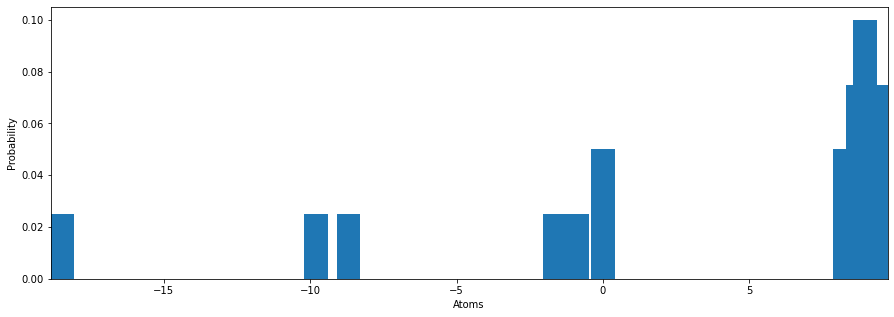
\includegraphics[height=0.2\textheight]{figures/personal_work/quantile.png}
    \caption{Example of a distribution projected with the quantile approach}
\end{figure}

This projection has the quality of being compatible with the Wasserstein metric, with which it gives a contracting operator.

\begin{proposition}
    $\Pi_{d_1}\TT^\pi$ is $\gamma$-contraction in $\overline{d}_\infty$ :

    \[ \overline{d}_\infty(\Pi_{d_1}\TT^\pi\eta_1 , \Pi_{d_1}\TT^\pi\eta_2) \leq \gamma \overline{d}_\infty(\eta_1, \eta_2)\]
\end{proposition}

This again leads to a convergence of the Bellman operator coupled with the projection step. However, no result have been found so far about a bound of distance between the true distribution of the policy and the policy it this operator converges to. The benefits of this projection is that it doesn’t require to have prior knowledge on the reward distribution, where the categorical approach requires bounds. It is thus more convenient to use.

% \subsubsection*{Diatomic AVaR}

% [Achab et Neu, motives about keeping the mean]

% \subsection{Quantile Optimization}


% Issues with greedy policy for implementation (Defourny 2008)    


% \subsubsection*{Quantile}

% [Morimura et al.]

% \subsubsection*{Superquantile}

% [results by Achab et Neu]


